\clearpage
\section{Auswertung}
\subsection{Zählrohrcharakteristik mit Natururan}
Um die Zählrohrcharakteristik mit Uran aufzunehmen, stellten wir einen Spannungsbereich von 1000 bis 4000 V ein. Die Schrittweite betrug 100 V. Als Messdauer stellten wir 50 s ein, als Einpendelzeit für die Spannung 15 s. Wir benutzten die gleichen Einstellungen, um den Untergrund zu vermessen. Mithilfe von LabView erhielten wir eine Zählrate n für jede Spannung. Deren Fehler $s_{n}$ berechnet sich wie folgt: \[n=\frac{N}{t},\] wobei N für die Anzahl der Counts und t für die Messdauer steht. \[\rightarrow s_{n}=\frac{\partial n}{\partial N}\cdot s_{N}=\frac{\sqrt{N}}{t}=\sqrt{\frac{n}{t}}.\] Dabei wird der Fehler der Zeit als vernachlässigbar angenommen. \\
Die resultierende Zählrate nach Abzug des Untergrunds (mit Countzahl U und Zählrate u) berechnet sich als \[n_{res}=\frac{N-U}{t}=\frac{N}{t}-\frac{U}{t}=n-u.\]
Da hier nicht davon ausgegangen werden kann, dass genug Counts gemessen wurden, um den Fehler des Untergrunds vernachlässigen zu können, gilt: \[s_{n_{res}}=\sqrt{(\frac{\partial n_{res}}{\partial n})^{2}\cdot s_{n}^{2}+\frac{\partial n_{res}}{\partial u}\cdot s_{u}^{2}}=\sqrt{\frac{n}{t}+\frac{u}{t}}.\] Für die Fehlerberechnungen wurde jeweils die Gauss'sche Fehlerfortpflanzungsmethode verwendet. Für die Zählrohrcharakteristik erhielten wir somit:
\begin{figure}[h]
\begin{center}
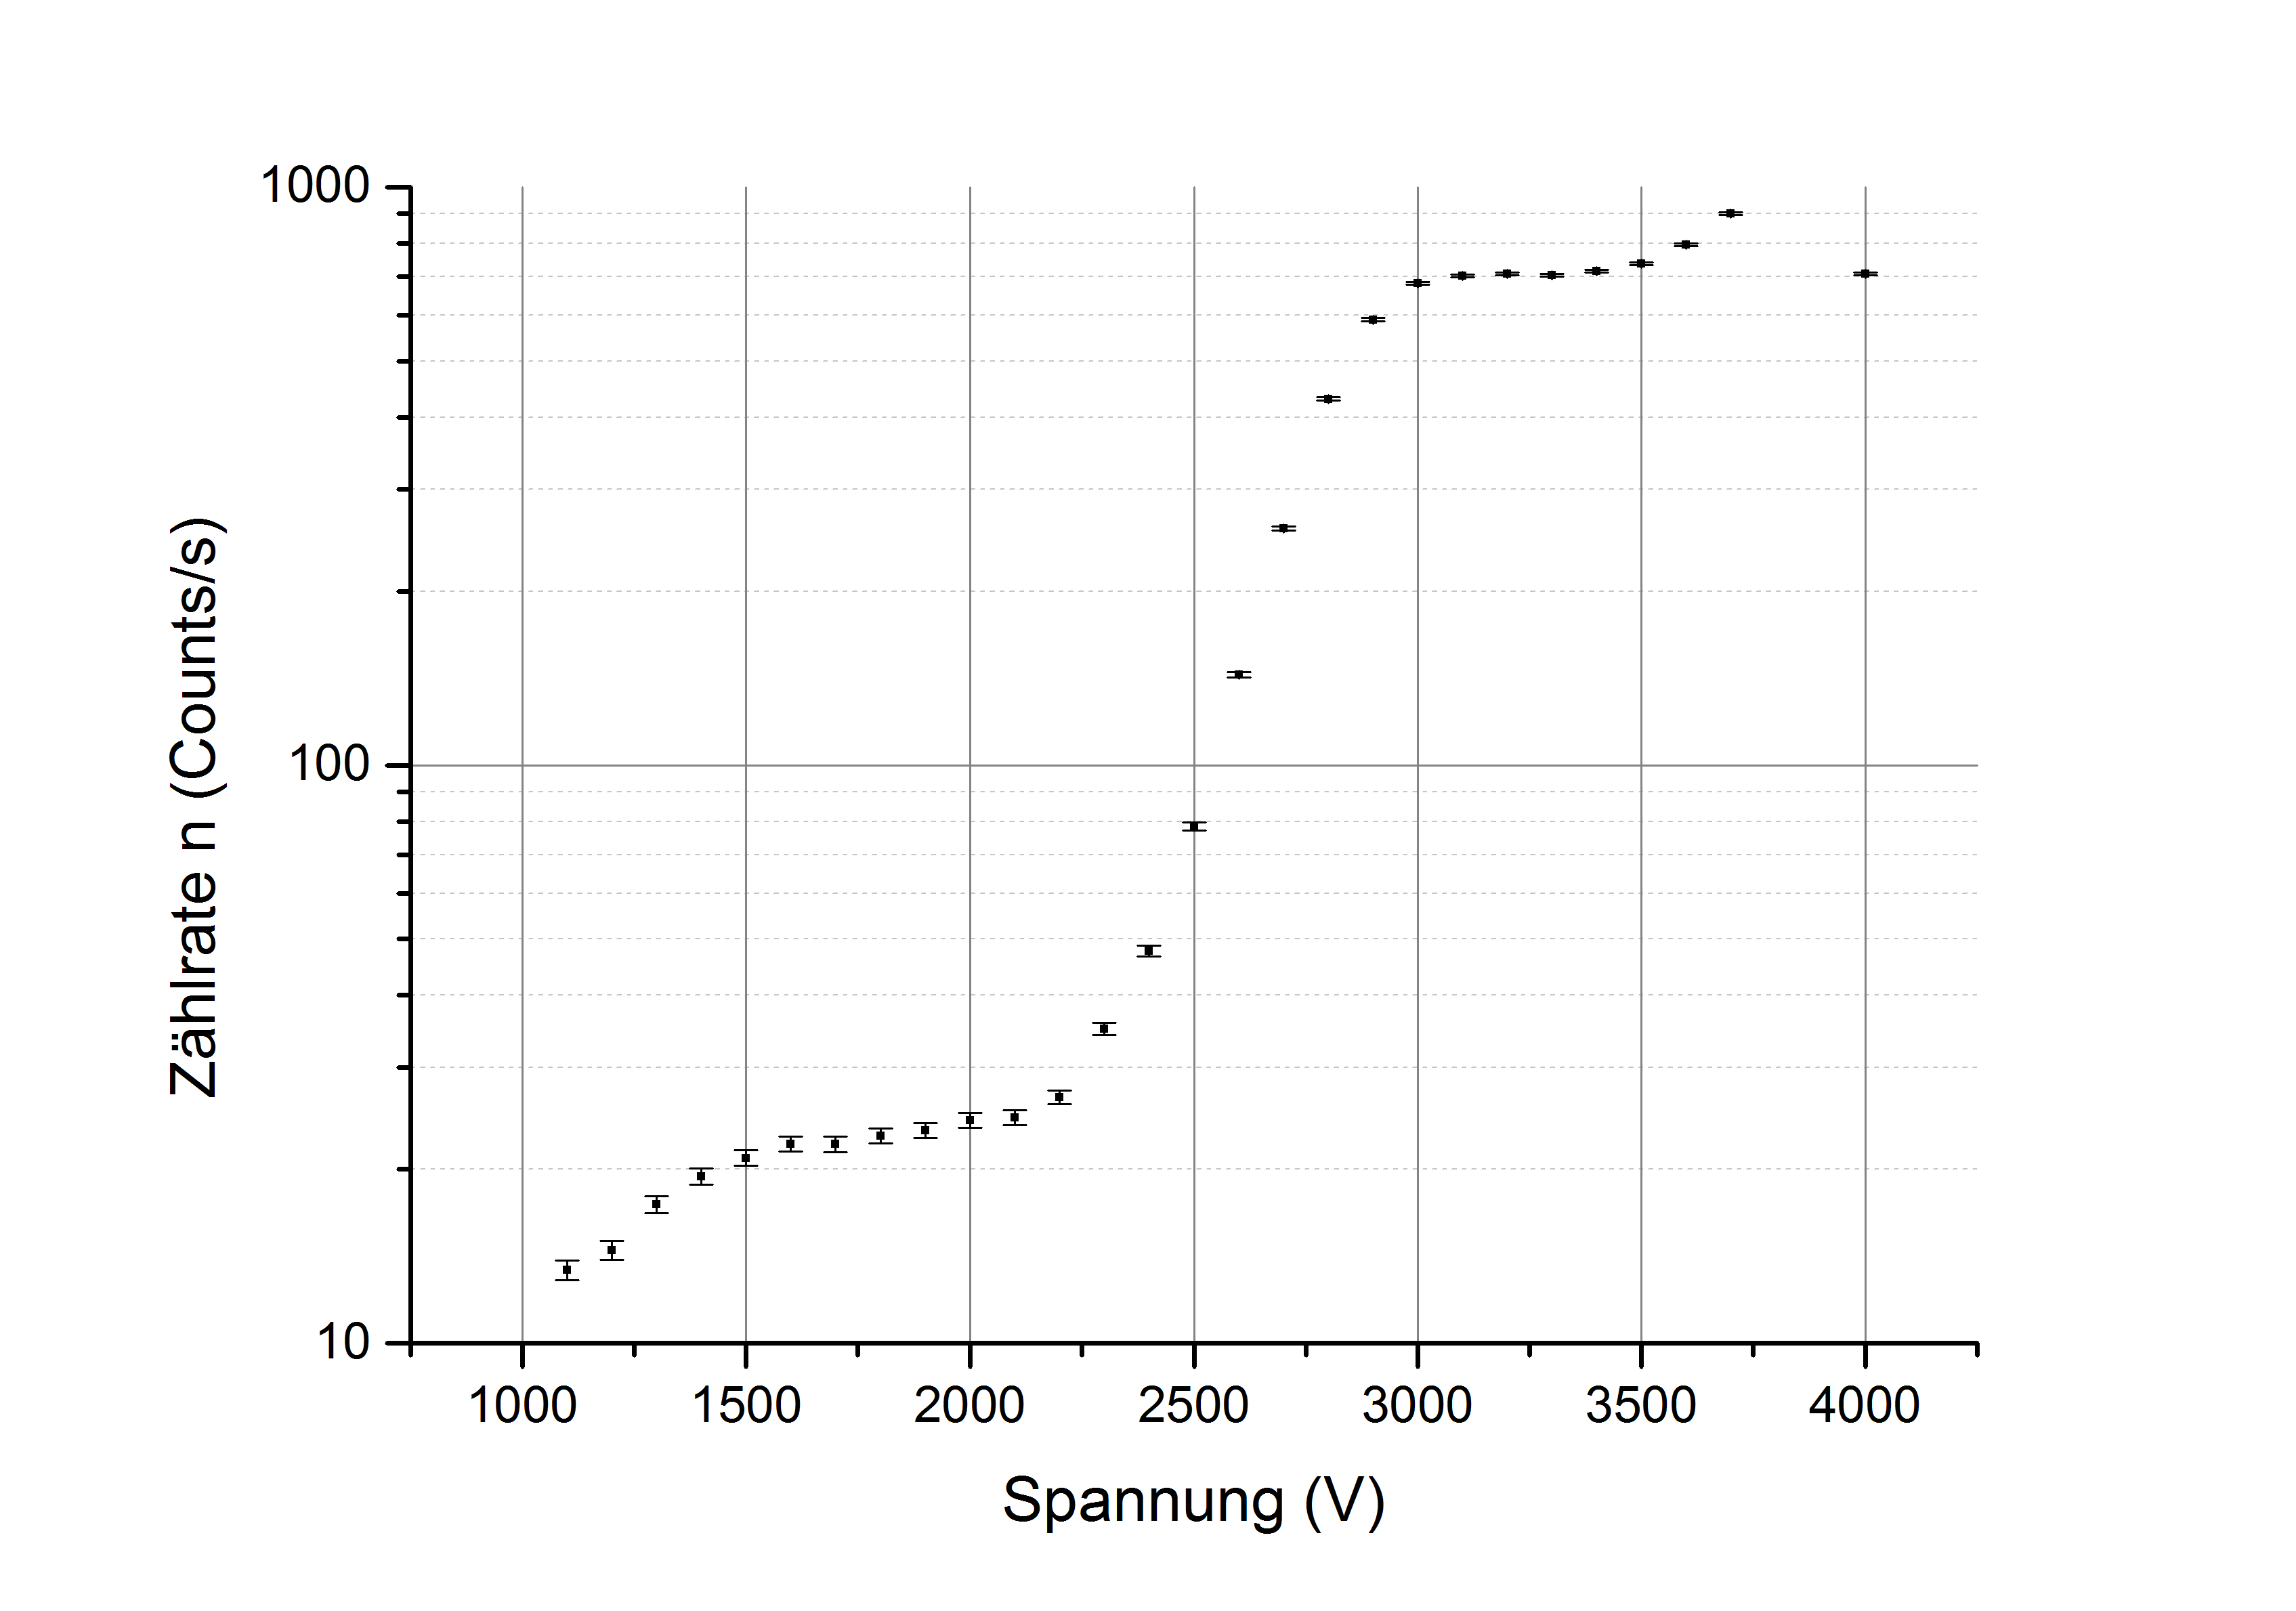
\includegraphics[scale=0.45]{Bilder/uranmess2}
\caption{Zählrohrcharakteristik, aufgenommen mit $^{238}U$, abzüglich des Untergrunds}
\end{center}
\end{figure}
~\\
Die Skalierung der y-Achse wählten wir logarithmisch, da sonst die Unterschiede bei den Zählraten bei niedrigen Spannungen nicht sichtbar wären. Der Fehler der Spannung wurde als vernachlässigbar angenommen.\\
Das $\alpha$-Plateau zeigte sich in dem Bereich zwischen 1600 und 2100 V, das $\beta$-Plateau zwischen 3100 und 3400 V.
\subsection{Bestimmung der Halbwertszeit von $^{40}K$}
Zunächst füllten wir ein Schälchen mit etwas KCl und vermaßen damit den Bereich zwischen 3000 und 4000 V, um die Arbeitsspannung zu bestimmen. Dabei wählten wir eine Messzeit von 100 s und eine Einpendelzeit von 20 s. Der Fehler auf die erhaltenen Zählraten berechnete sich zu $s_{n}=\sqrt{\frac{n}{t}}$, wie bereits im Unterkapitel für Natururan diskutiert.  Wir erhielten folgenden Verlauf:
\begin{figure}[h]
\begin{center}
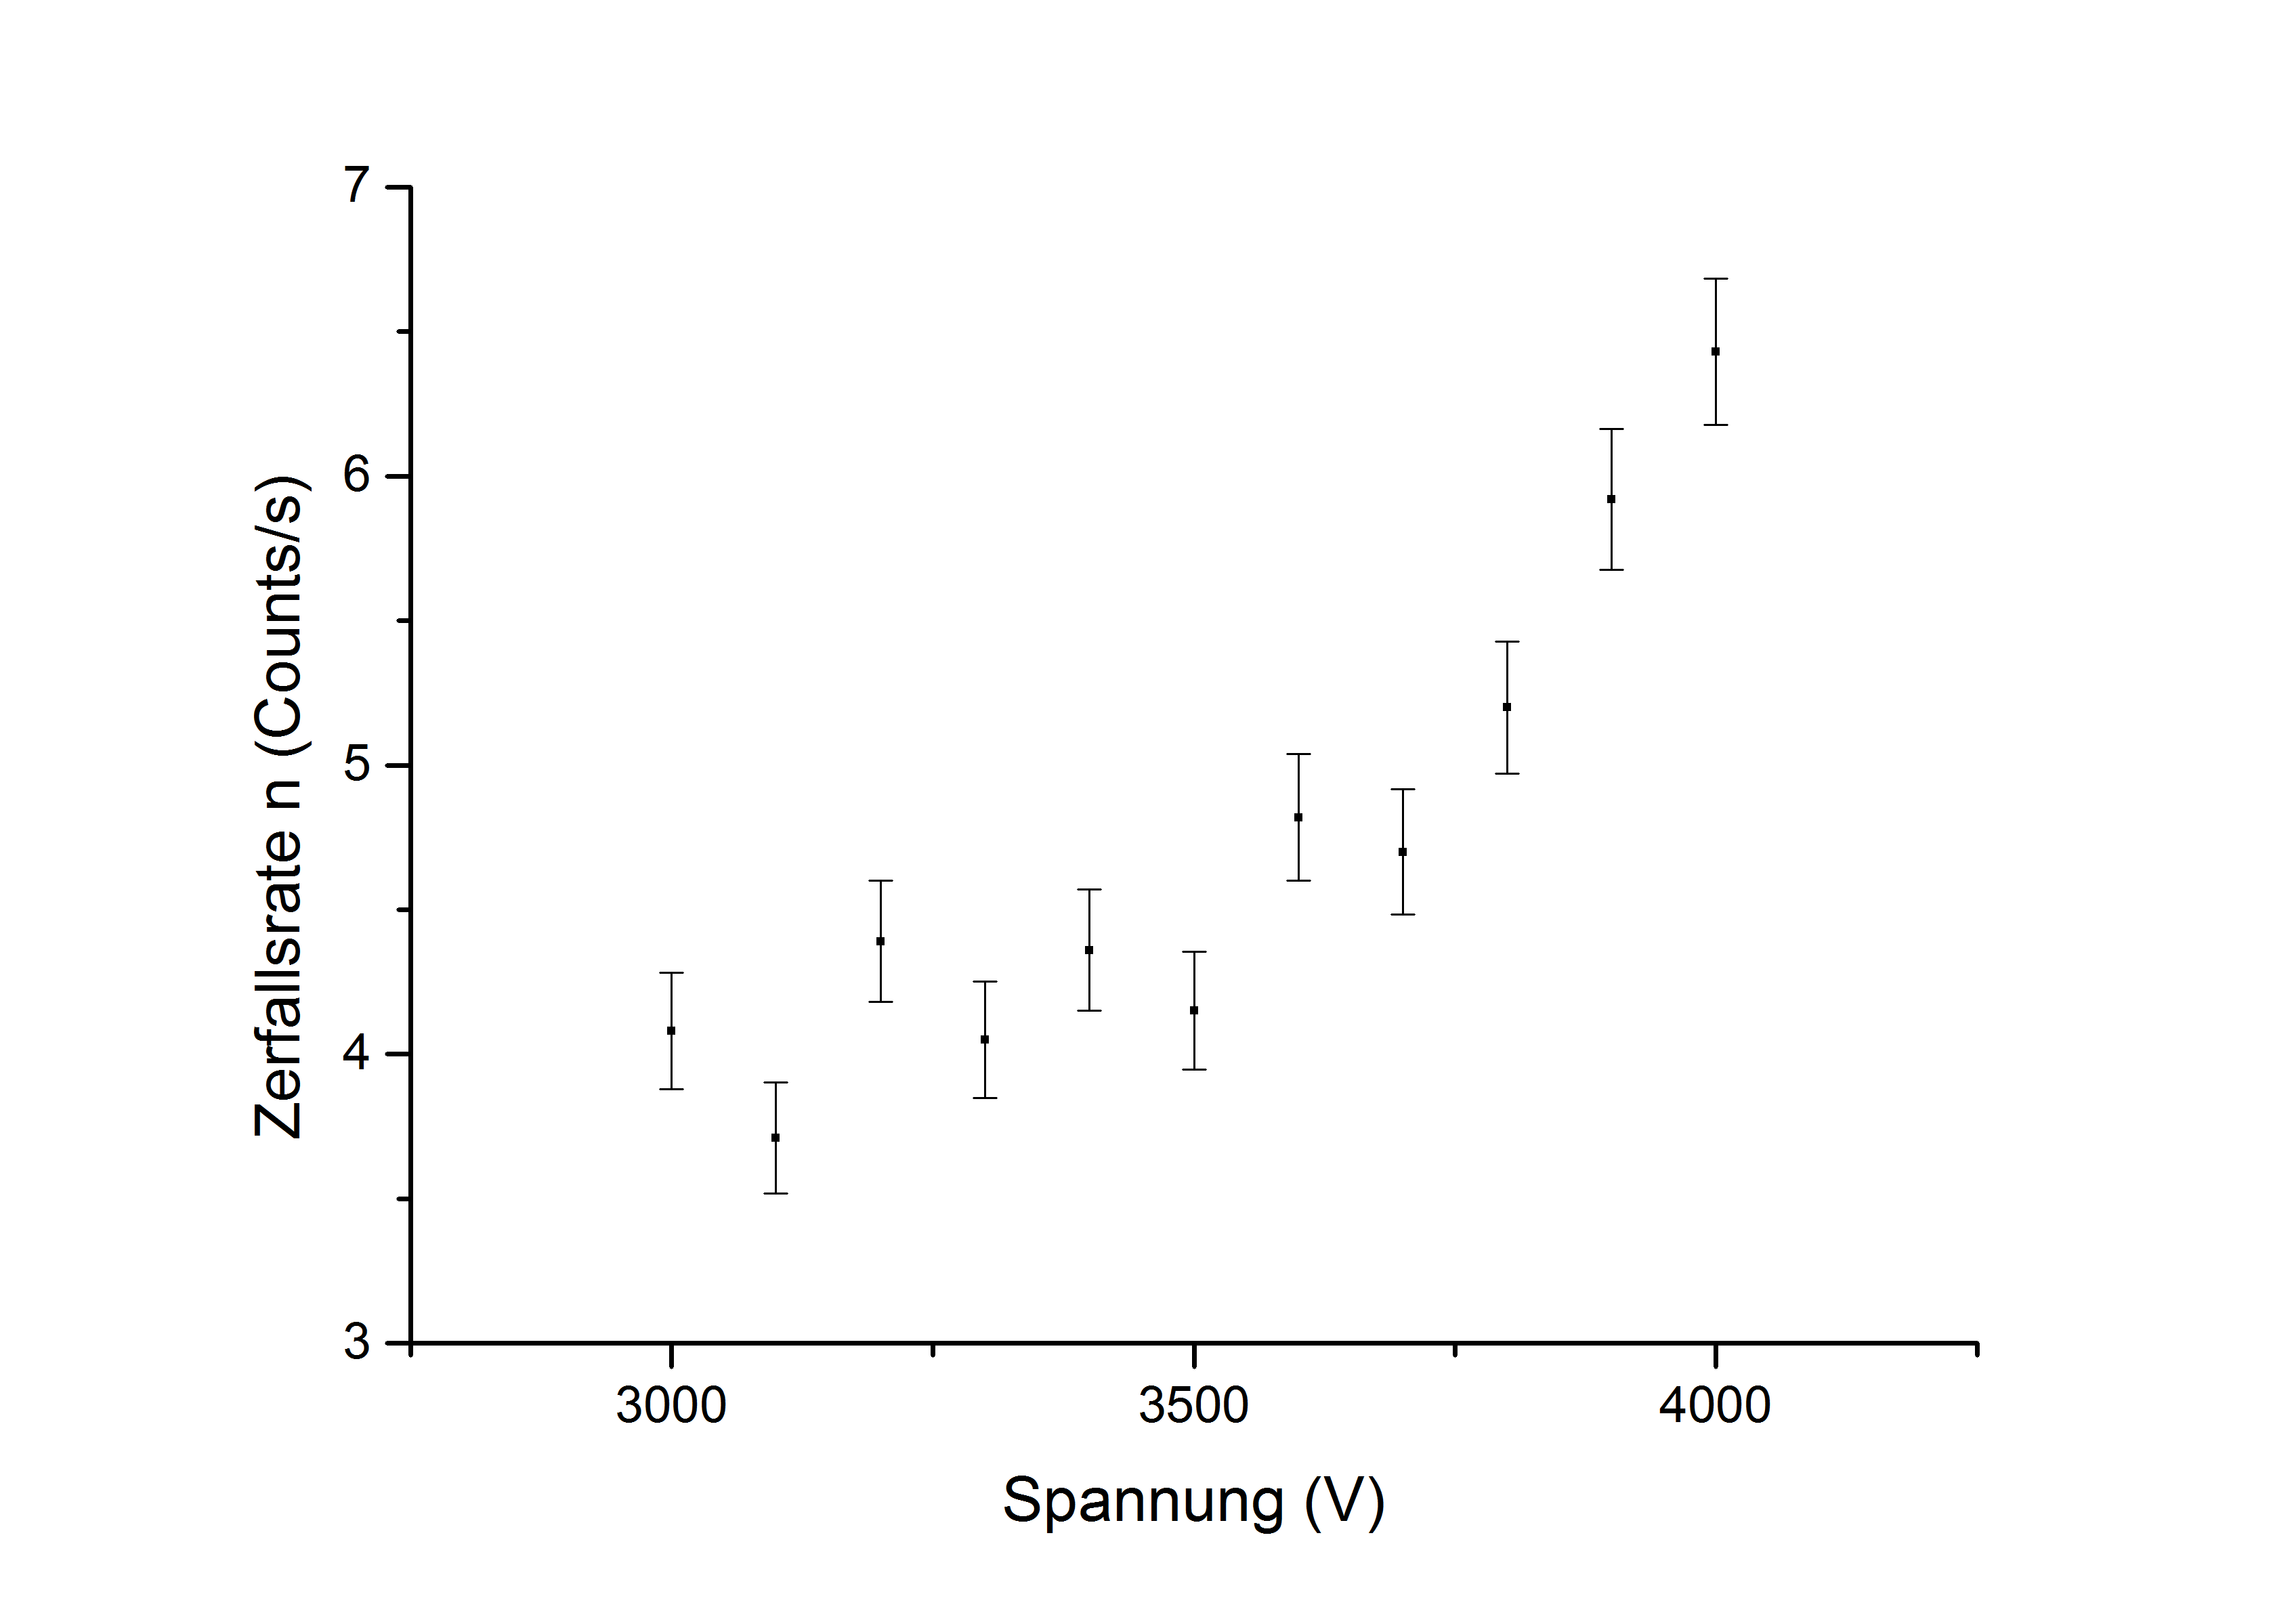
\includegraphics[scale=0.4]{Bilder/apkalium}
\caption{Vermessung des Plateaus von $^{40}K$}
\end{center}
\end{figure}
~\\
Aufgrund des erhaltenen Verlaufs entschieden wir uns für eine Arbeitsspannung von $U_{AP}=3200V$.\\
Um eine Messdauer zu bestimmen, für welche der relative Fehler der Zählrate bei 2\% liegt, füllten wir sehr wenig KCl-Pulver ($m=(0,1614\pm0,0001)g$), wobei die Waage auf die Masse des Aluminiumschälchens geeicht wurde, sodass nur die Masse des Pulvers angezeigt wurde. Als Fehler wurde die letzte Stelle der Anzeige angenommen. Als Zählrate erhielten wir bei einer Messdauer von $t=200s$ $n=(2,15\pm0,10)\frac{Counts}{s}$. Mithilfe dieses Ergebnisses wurde die Messdauer mithilfe der Formel $t=\frac{2500}{n}$ (s. 'Theoretische Grundlagen') bestimmt. Der Fehler berechnet sich mithilfe der Gauss'schen Fehlerfortpflanzung somit zu $s_{t}=\left|\frac{\partial t}{\partial n}\right|\cdot s_{n}=\frac{2500}{\sqrt{n^{3}\cdot t}}$. Somit erhielten wir für die Messdauer $t=(1160\pm60)s$. Somit entschieden wir uns für eine Messdauer von $t=1200s$. Da die Wahl mit einer sehr geringen Masse und damit einer geringen Zählrate stattfand, konnte gewährleistet werden, dass der relative Fehler die Vorgaben erfüllte. \\
Lediglich für die Masse von $m=(0,0988\pm0,0001)g$ wurde eine höhere Messdauer von $t=1800 s$ gewählt, da hier eine geringere Zählrate als für die Messung, mithilfe derer die Wahl fiel, zu erwarten war (aufgrund der geringeren Messung). \\
Vor dem Start der Messungen bestimmten wir die Zählrate auch für $m=(1,6625\pm0,0001)g$, also einem vollen Schälchen, und erhielten  eine Zählrate von $n=(5,73\pm0,17)\frac{Counts}{s}$ und damit analog zu der vorangegangenen Rechnungen eine Zeit von $t=(437\pm13)s$, weshalb wir für die letzten beiden Messungen mit Massen von $m=(1,6256\pm0,0001)g$ und $m=(1,6604\pm0,0001)g$ eine Messdauer von lediglich $t=500s$ wählten. \\
Bei der Einstellung der Messdauer für die Untergrundmessung erhielten wir nach mehrfacher Messung eine Zählrate von $n\approx 0,5 \frac{Counts}{s}$. Somit bestimmten wir als Messdauer $t=20000s$. Um sicher zu gehen, dass genug Counts gemessen werden und um das ganze Wochenende auszunutzen, vermaßen wir den Untergrund von 2900-3800 V in 100 V-Schritten, wobei wir eine Messdauer von $t=6h=21600s$ pro Schritt und eine Einpendelzeit von 5 Minuten wählten. Um überprüfen zu können, dass alles in Ordnung lief und es zu keinen extremen Ausreißern oder Verfälschungen des Ergebnisses durch beispielsweise einen nicht konstanten Gasdruck kam, ließen wir die Zählrate alle 10 Minuten anzeigen. An der Berechnung für den Fehler der Zählrate, $n=\sqrt{\frac{n}{t}}$, wobei $n=\frac{n_{1}+...n_{m}}{m}$ der Mittelwert der m angezeigten Zählraten und t die Messdauer für einen Schritt ist, ändert dies nichts, da gilt:
 \[s_{n}=\sqrt{(\frac{\partial n}{\partial n_{1}})^{2}\cdot s_{n_{1}}^{2}+...+(\frac{\partial n}{\partial n_{m}})^{2}\cdot s_{n_{m}}^{2}}=\sqrt{\frac{s_{n_{1}}^{2}}{m^{2}}+...+\frac{s_{n_{m}}^{2}}{m^{2}}}=\]
 \[\frac{1}{m}\sqrt{\frac{n_{1}}{\left(t/m\right)}+...+\frac{n_{m}}{\left(t/m\right)}}=\sqrt{\frac{n_{1}+...+n_{m}}{m}}\cdot\sqrt{\frac{1}{t}}=\sqrt{\frac{n}{t}}.\]
 Für die resultierende Gesamtrate, also der gemessenen Rate n abzüglich der Untergrundrate u erhalten wir somit: \[n_{res}=n-u\] mit dem statistischen Fehler \[s_{n_{s}}=\sqrt{s_{n}^{2}+s_{u}^{2}}=\sqrt{\frac{n}{t_{n}}+\frac{u}{t_{u}}},\] wobei $t_{n}$ für die jeweilige Messdauer mit KCl-Pulver und $t_{u}$ für die Messdauer für den Untergrund steht.\\
 Um den Fehler besser abschätzen zu können, nahmen wir die Messung für $m=1,5306g$ doppelt vor. Dabei erhielten wir $n_{1}=(5,37\pm0,07)\frac{Counts}{s}$ bzw. $n_{2}=(5,39\pm0,07)\frac{Counts}{s}$. Die Werte sind im Rahmen der Messungenauigkeit gleich. Dennoch entschlossen wir uns, die Hälfte der Differenz der gemessenen Raten als Fehler $s_{n_{diff}}=0,01\frac{Counts}{s}$ zu berücksichtigen, um ein möglichst genaues Ergebnis zu erhalten. \\
 Der resultierende Fehler kann jetzt bestimmt werden zu \[s_{n_{res}}=\sqrt{s_{n_{diff}}^{2}+s_{n_{s}}^{2}}.\]
 Für den Untergrund erhielten wir am Arbeitspunkt eine Rate von $u=(0,568\pm0,005)\frac{Counts}{s}$. Der relative Fehler beträgt 0,9\%, was geringer als gefordert ist, da die Zeit höher als die berechneten 20000 s gewählt wurde und die Rate höher als die $0,5 \frac{Counts}{s}$ ist, mit denen wir rechneten. Der Fehler auf den Untergrund kann somit vernachlässigt werden.
 \clearpage
 Wir trugen die resultierende Zählrate über die benutzten Massen auf und fitteten die in den 'Theoretischen Grundlagen' diskutierte Funktion $n(m)=a(1-e^{-bm})$ an den Verlauf:
 \begin{figure}[h]
 \begin{center}
 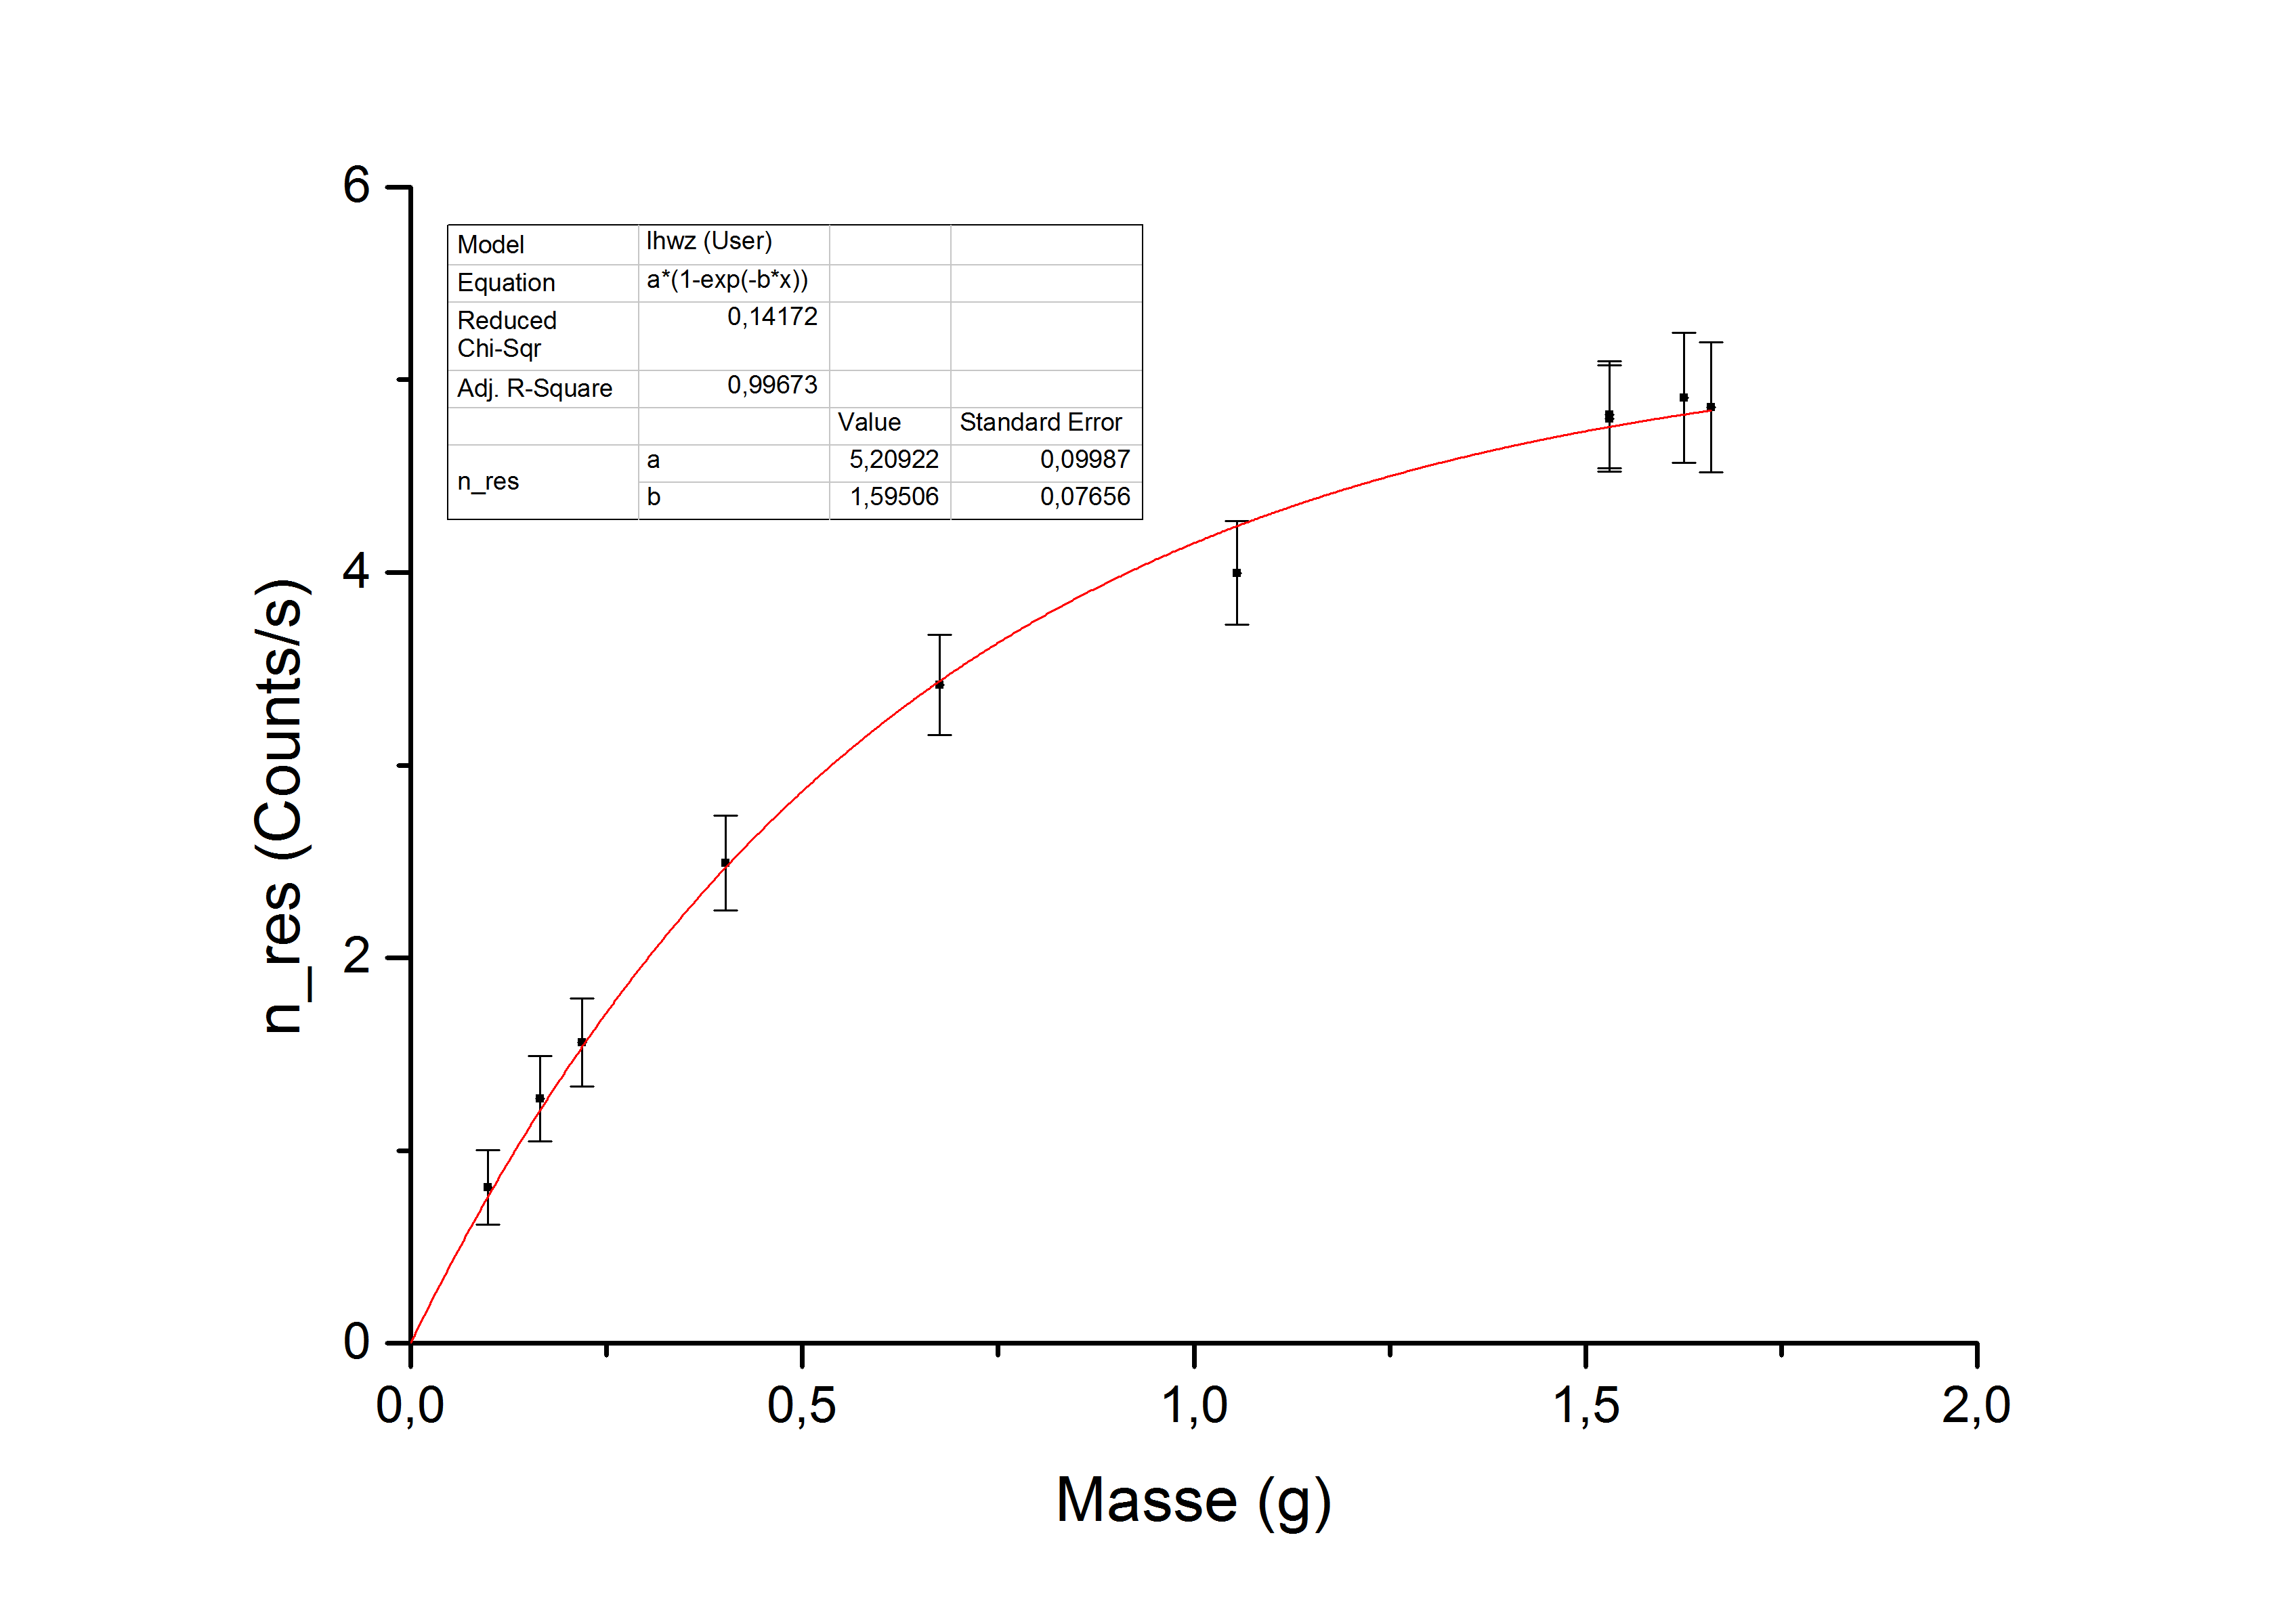
\includegraphics[scale=0.6]{Bilder/kalium}
 \caption{Massenabhängige Messung der Zerfallsraten für $^{40}K$ mit Fitfunktion}
 \end{center}
 \end{figure}
 ~\\
 Die Fehlerbalken in x-Richtung sind nicht sichtbar, da die Messfehler auf m sehr klein sind.\\
 Wie der Wert $\frac{\chi^{2}}{Anzahl der Freiheitsgrade}=0,14172$, welcher sehr gering ist, zeigt, beschreibt der Fit den Verlauf sehr gut. Andersherum kann man sagen, dass unsere Messergebnisse den theoretischen Verlauf bestätigen. Auch das korrigierte Bestimmtheitsmaß ('Adjusted R-Square'), welches 0,99673 beträgt, zeugt von einer sehr guten Anpassung, da ein Wert von 1 eine perfekte Übereinstimmung von Fit und Werten anzeigt und die Differenz zwischen diesem und dem mithilfe unseres Fits bestimmten Wert sehr klein ist. \\
 Für die Parameter a und b erhielten wir folgende Werte: \[a=(5,21\pm0,10)\frac{Counts}{s}\]
 \[b=(1,60\pm0,08)g^{-1}.\]  Für die Kovarianzmatrix C ergibt sich:
  \[C=\begin{pmatrix} s_{a}^{2} & cov(a,b) \\ cov(a,b) & s_{b}^{2} \\  \end{pmatrix}=\begin{pmatrix} 0,00997 & -0,00667 \\ -0,00667 & 0,00586 \\  \end{pmatrix}.\] 
  Damit ergibt sich für die spezifische Aktivität \[A_{s}=\frac{2ab}{f_{B}}=12,88 \frac{Counts}{s\cdot g}.\] 
  Der Fehler der spezifischen Aktivität, $s_{A_{s}}$, berechnet sich aufgrund der Kovarianz durch \[s_{A_{s}}=\sqrt{\left(\frac{\partial A_{s}}{a}\right)^{2}s_{a}^{2}+\left(\frac{\partial A_{s}}{\partial b}\right)^{2}s_{b}^{2}+2\left(\frac{\partial A_{s}}{\partial a}\right)\cdot\left(\frac{\partial A_{s}}{\partial b}\right)cov(a,b)}=\]
  \[A_{s}\cdot\sqrt{\left(\frac{s_{a}}{a}\right)^{2}+\left(\frac{s_{b}}{b}\right)^{2}+\frac{2cov(a,b)}{ab}}=0,42 \frac{Counts}{s\cdot g}.\] 
  ~\\
  Insgesamt erhält man für die spezifische Aktivität somit $A_{s}=(12,9\pm0,4)\frac{Counts}{s\cdot g}$.\\
  Die Halbwertszeit berechnet sich dann durch die Formel (s. 'Theoretische Grundlagen') \[T_{1/2}=\frac{ln(2)\cdot h_{rel}N_{A}}{1,12\cdot m_{rel_{KCl}}A_{s}}=4,58\cdot10^{16}s=1,45\cdot10^{9}a.\] Dabei haben wir angenommen, dass ein Jahr im Mittel 365,25 Tage hat.\\
  Da $A_{s}$ die einzige als fehlerbehaftet angenommene Größe in der Formel für die Halbwertszeit ist, gilt für deren Fehler mithilfe Gauss'scher Fehlerfortpflanzung: 
  \[s_{T_{1/2}}=T_{1/2}\cdot\frac{s_{A_{s}}}{A_{s}}=4,7\cdot10^{7}a.\] 
  Insgesamt erhalten wir damit für die Halbwertszeit: \[T_{1/2}=(1,45\pm0,05)\cdot10^{9}a.\] 
  Der Literaturwert beträgt $T_{1/2,lit}=1,28\cdot10^{9}a$. Der mithilfe unserer Messwerte ermittelte Wert liegt innerhalb von $4\sigma$ auf diesem. Es ist möglich, dass die untere Schwelle leicht zu hoch gewählt war, wodurch die Zählrate zu niedrig und die Halbwertszeit zu hoch bestimmt würde. Weiterhin ist zu beachten, dass das verwendete KCl-Pulver nicht absolut rein war, weshalb die tatsächliche Masse an KCl geringer sein sollte, wodurch die spezifische Aktivität höher und damit die Halbwertszeit kleiner als bestimmt ist. Außerdem wird der Rückstreufaktor am Aluminium-Schälchen als konstant angenommen, wobei die Dicke der Probe, also die Höhe, in der das Pulver aufgehäuft ist, keine Rolle spielt. Eigentlich spielt diese jedoch eine Rolle und sorgt bei ihrer Erhöhung für ein höheres Maß an Selbstabsorption, was zu einer zu niedrig bestimmten Schranke der Zählrate führt. Diese wiederum ist proportional zur spezifischen Aktivität, welche antiproportional zur Halbwertszeit ist. Alles in allem führt führt dies also zu einer zu einer zu hoch bestimmten Halbwertszeit, welche tatsächlich niedriger sein sollte. 
  \clearpage
  \subsection{Bestimmung der Halbwertszeit von $^{147}Sm$}
  Zunächst bestimmten wir die Position des $\alpha$-Plateaus, indem wir die Spannungen im Bereich von 1200 bis 2700 V in 100 V-Schritten durchfuhren. Die Messdauer betrug dabei $t=200s$, die Einpendelzeit für die Spannungen 20 s. Der Fehler der Zählraten wurde, wie bereits diskutiert, durch $s_{n}=\sqrt{\frac{n}{t}}$ berechnet. Die Einengung der vermessenen Spannungen nahmen wir mithilfe der für Natururan aufgenommenen Zählrohrcharakteristik vor. Wir erhielten somit folgenden Verlauf:
  \begin{figure}[h]
  \begin{center}
  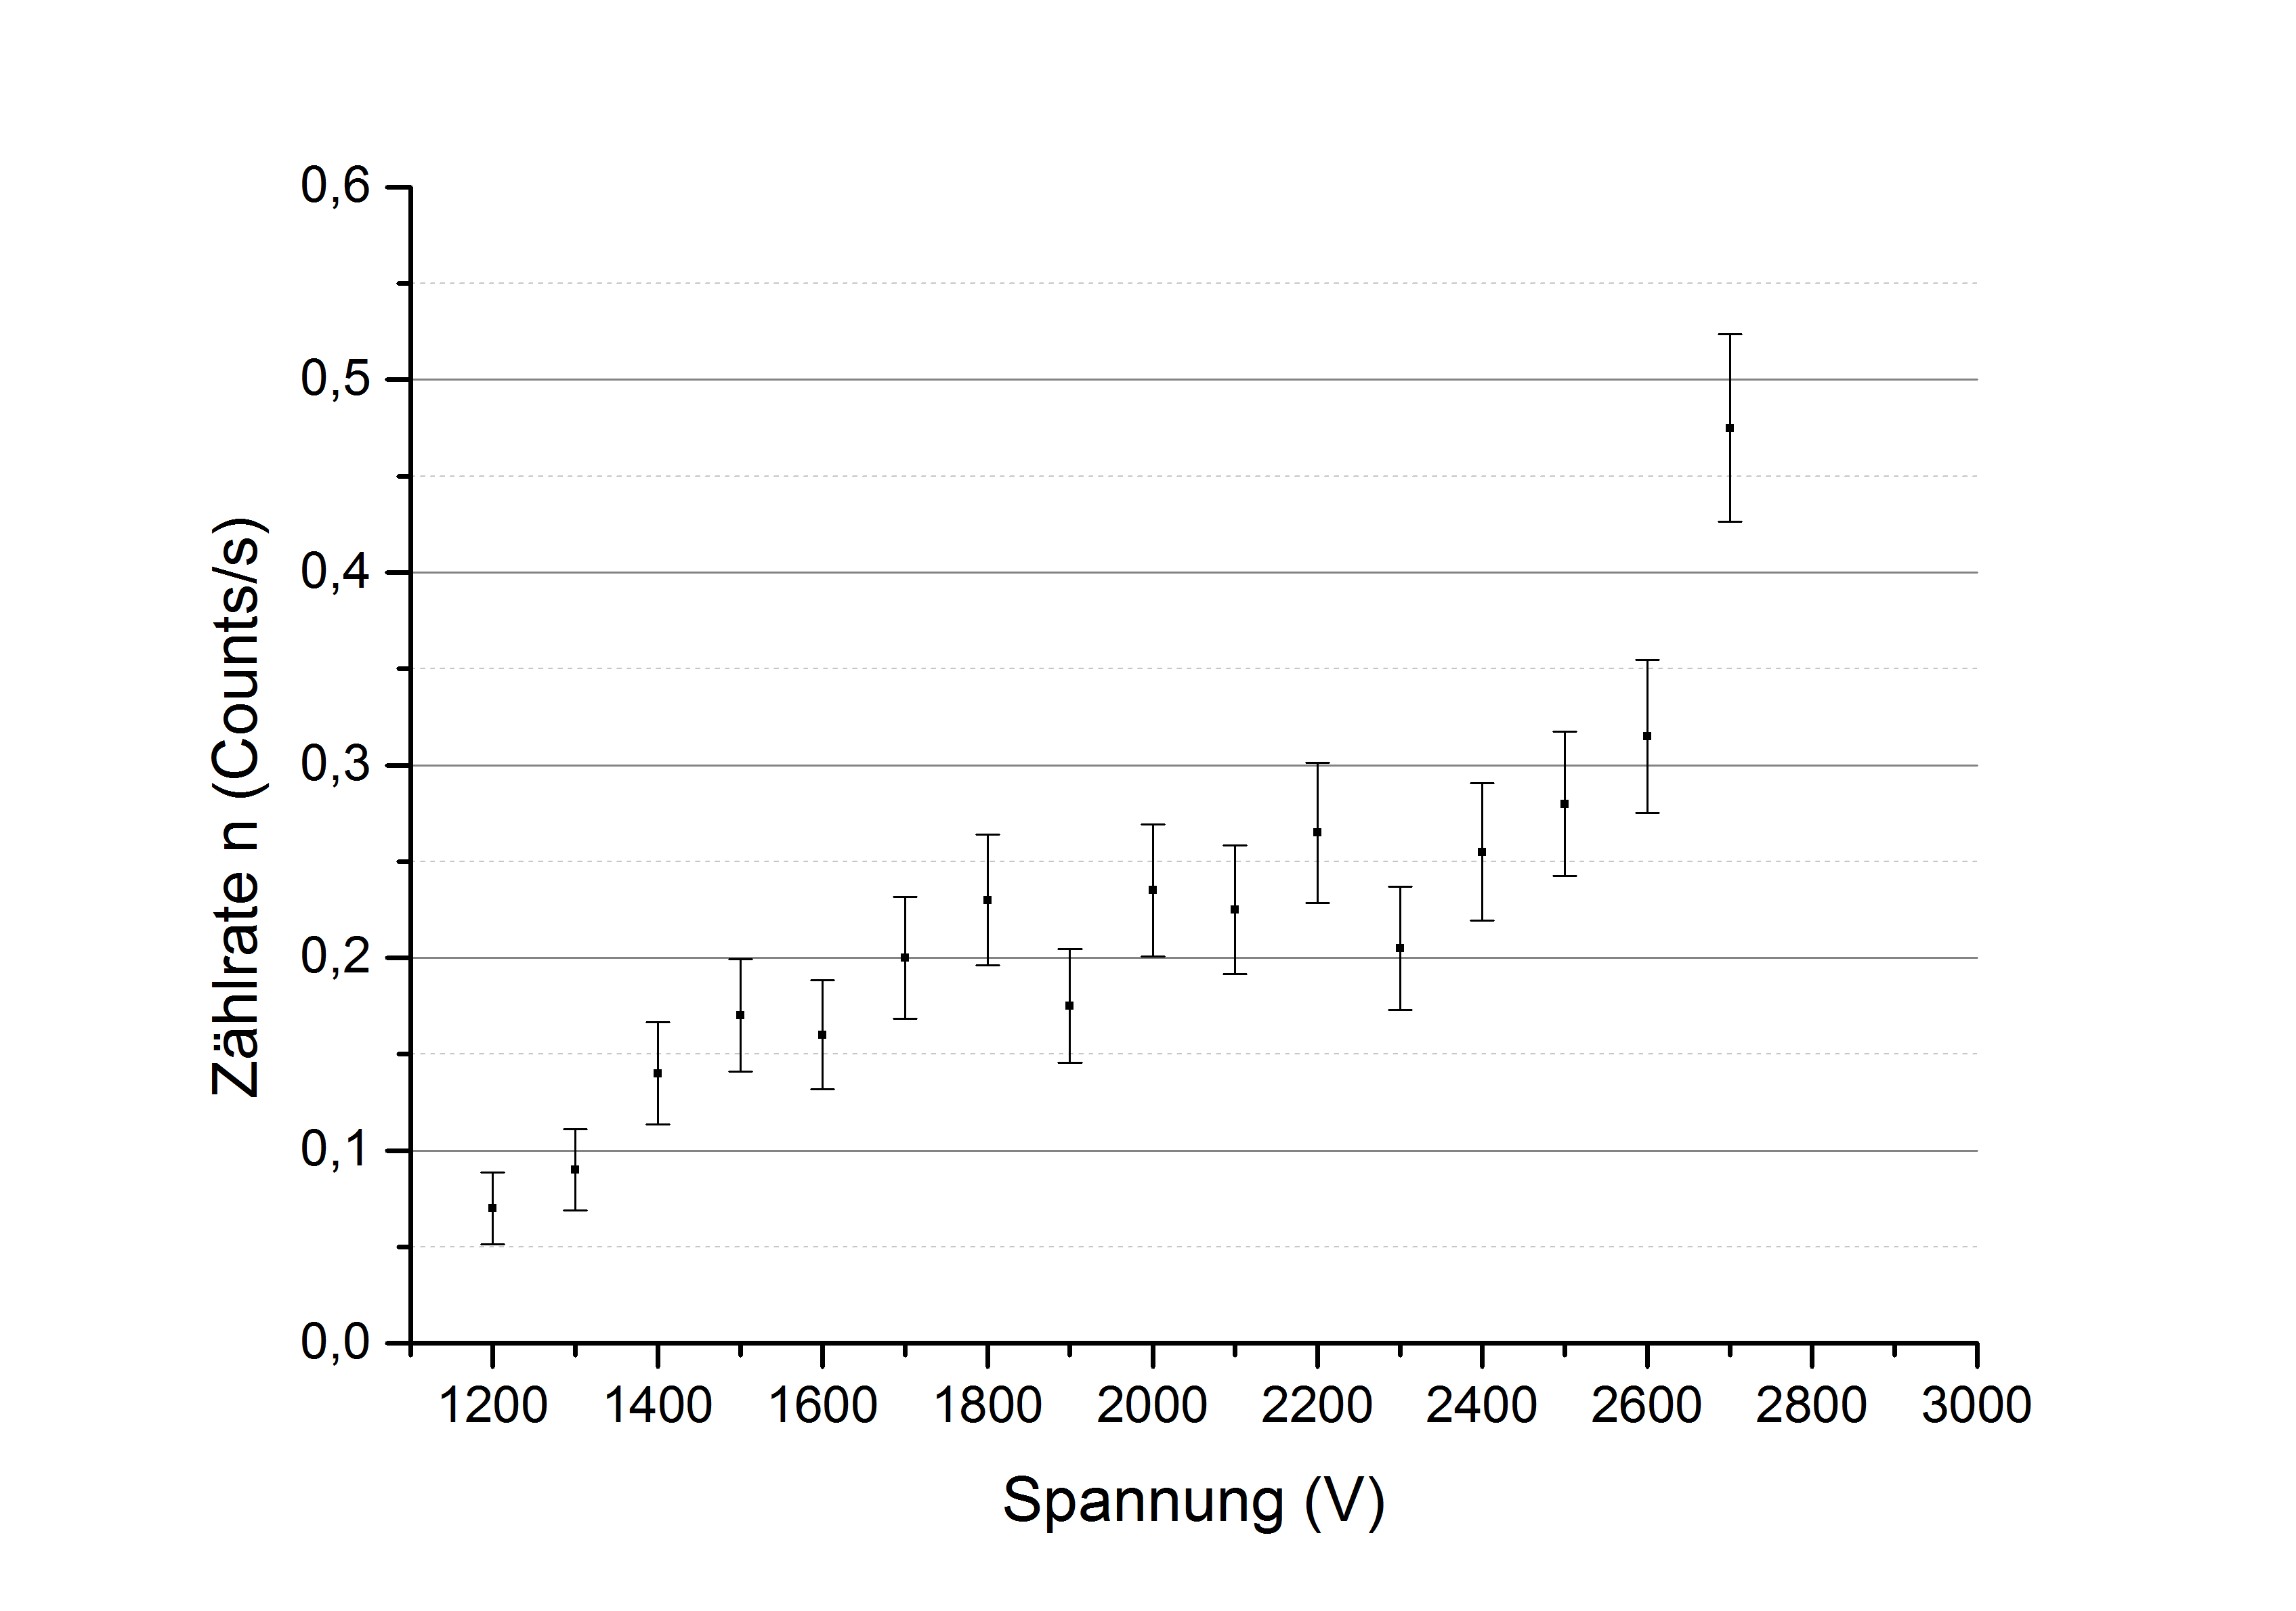
\includegraphics[scale=0.5]{Bilder/smlin}
  \caption{Aufnahme des $\alpha$-Plateaus für $^{147}Sm$}
  \end{center}
  \end{figure}
  ~\\
  Das $\alpha$-Plateau ist in dem Bereich zwischen 1700 und 2300 V. Als Arbeitspunkt wählten wir somit $U_{AP}=2000 V$.\\
  Da die gemessenen Zählraten sehr niedrig waren, musste die untere Grenze verändert werden, ab welcher Counts detektiert werden. Wir veränderten diese so, dass der Untergrund eine Rate von $u=(0,27\pm0,04)\frac{Counts}{s}$ aufwies (am Arbeitspunkt, bestimmt mit einer Messdauer von $t=200s$). \\
  Danach füllten wir eine Aluminiumschale mit kleiner Oberfläche (Durchmesser $d=(1,695\pm0,005)cm$ - der Fehler ergab sich dadurch, dass es uns nicht möglich war, genauer als auf die halbe Distanz zwischen zwei Markierungen am Messschieber abzulesen) und vermaßen die Zerfallsrate mit derselben Messdauer wie den Untergrund. Als Ergebnis erhielten wir $n=(0,95\pm0,07)\frac{Counts}{s}$. Damit berechneten wir die Messdauer, um einen relativen Fehler von 2\% zu erhalten, zu $t=\frac{2500}{n}=2631,6s$. Der Fehler auf diese Größe berechnete sich mit Gauss'scher Fehlerfortpflanzung analog zum vorigen Kapitel zu $s_{t}=190,9s$. Wir wählten die Messdauer schließlich als $t=2700 s$, um möglichst Zeit zu sparen. \\
  Als Resultat dieser Messung erhielten wir eine Zerfallsrate von $n=1,704\frac{Counts}{s}$, mitsamt des Fehlers also $n=(1,70\pm0,03)\frac{Counts}{s}$. Da die mithilfe der kurzen Messzeit bestimmte Zählrate deutlich zu gering war, reichte also die Messdauer von $t=2700 s$ völlig aus. Der relative Fehler betrug somit nur 1,47\%.\\
  Sinnvolle Messungen mit anderen Oberflächen erwiesen sich als unmöglich, da plötzlich selbst ohne Gasdruck und Probe Zerfallsraten von $n=70\frac{Counts}{s}$ und mehr gemessen wurden, was nur auf ein gravierendes Problem im Aufbau hinweisen kann. Vermutlich war die Elektronik aufgrund des tagelangen Dauereinsatzes nicht mehr einsatzfähig.\\
  Aus diesem Grund kann die Auswertung nur mit dem einen ermittelten Wert und der Untergrundmessung, welche sehr kurz vorgenommen wurde, um die untere Grenze einzustellen, erfolgen. Wegen der kurzen Messdauer kann der Fehler auf die Rate des Untergrunds nicht vernachlässigt werden. \\
  ~\\
  Die tatsächliche Zerfallsrate wurde analog zum vorherigen Kapitel berechnet durch \[n_{res}=n-u=1,434\frac{Counts}{s}.\] 
  Der Fehler ergab sich zu \[s_{n_{res}}=\sqrt{s_{n}^{2}+s_{u}^{2}}=0,0445\frac{Counts}{s}.\]
  Insgesamt erhält man also \[n_{res}=(1,43\pm0,04)\frac{Counts}{s}.\]
  Wie bereits in dem Kapitel 'Theoretische Grundlagen' beschrieben, hängt die Halbwertszeit von der Fläche und der Zerfallsrate ab. Die Fläche berechnet sich, da die Oberfläche kreisförmig ist, als \[F=\left(\frac{d}{2}\right)^{2}\cdot\pi.\] Der Fehler berechnet sich als \[s_{F}=\frac{\partial F}{\partial d}\cdot s_{d}=\frac{\pi}{2}\cdot d s_{d}.\]
  Für die Fläche erhalten wir mit dem bereits erwähnten Durchmesser von $d=(1,695\pm0,005)cm$ somit \[F=(2,256\pm0,013)cm^{2}.\] 
  Mithilfe dieser Werte kann die Halbwertszeit durch die in den 'Theoretischen Grundlagen' diskutierte Formel \[T_{1/2}=\frac{ln(2)R_{Sm_{2}O_{3}}\cdot\rho_{Sm_{2}O_{3}}\cdot N_{A}h_{rel}}{2m_{rel_{Sm_{2}O_{3}}}}\cdot\frac{F}{n_{res}}\] berechnet werden. Der Fehler berechnet sich zu
   \[s_{T_{1/2}}=\sqrt{\left(\frac{\partial T_{1/2}}{\partial F}\right)^{2}s_{F}^{2}+\left(\frac{\partial T_{1/2}}{\partial n_{res}}\right)^{2}s_{n_{res}}^{2}}=\]
   \[T_{1/2}\sqrt{\left(\frac{s_{F}}{F}\right)^{2}+\left(\frac{s_{n_{res}}}{n_{res}}\right)^{2}}.\] 
   Somit wurde die Halbwertszeit zu \[T_{1/2}=(0,179\pm0,005)\cdot10^{11}a\] bestimmt. Dieser Wert liegt weit von dem in [ver] gegebenen Literaturwert $T_{1/2,lit}=1,06\cdot10^{11}a$ entfernt.\\
   Dies kann zahlreiche Ursachen haben: Die Oberfläche der Probe war nicht perfekt kreisförmig, sondern leicht uneben, wodurch die tatsächliche Oberfläche und damit die Halbwertszeit größer als gemessen war. Natürlich kann aber dies kein Grund für unsere Abweichung vom Literaturwert sein, da diese viel zu groß ist, um eine solch geringfügige Ursache zu haben. \\
   Es ist möglich, dass die Diskriminatorschwelle zu niedrig gewählt wurde, weshalb eine höhere Zählrate gemessen wurde, was aufgrund der Antiproportionalität von Zählrate und Halbwertszeit zu einer Verkleinerung dieser führen kann. Wir gehen allerdings davon aus, dass die Einstellung in Ordnung war, da die erste Messung für den Untergrund ein sinnvolles Ergebnis ergab.\\
   Am wahrscheinlichsten ist es daher, dass bereits bei den von uns zunächst als sinnvoll erachteten Messungen zu viele Counts registriert wurden, was die Zählrate erhöht und die Halbwertszeit verkleinert. Ein Indiz hierfür ist, dass die erste Messung mit der Probe, aufgrund welcher wir die Messdauer bestimmten, eine deutlich niedrigere Zählrate als die darauffolgende, lange Messung aufwies. Wahrscheinlich wurden daher schon in letzterer Messung zu viele Counts registriert.